\documentclass[10pt,twoside]{article}
\usepackage[utf8]{inputenc}
\usepackage{amsmath}
\usepackage{amsfonts}
\usepackage{amssymb}
\usepackage[spanish,es-noshorthands]{babel}
\usepackage[T1]{fontenc}
\usepackage{lmodern}
\usepackage{graphicx,hyperref}
\usepackage{tikz,pgf}
\usepackage{multicol}
\usepackage{subfig}
\usepackage[papersize={6.5in,8.5in},width=5.5in,height=7in]{geometry}
\usepackage{fancyhdr}
\pagestyle{fancy}
\fancyhead[LE]{
\includegraphics[height=12pt]{Images/logo-colegio.png} Aritmética $6^{\circ}$}
\fancyhead[RE]{}
\fancyhead[RO]{\textit{Germ\'an Avenda\~no Ram\'irez, Lic. U.D., M.Sc. U.N.}}
\fancyhead[LO]{}

\author{Germ\'an Avenda\~no Ram\'irez, Lic. U.D., M.Sc. U.N.}
\title{\begin{minipage}{.2\textwidth}

\includegraphics[height=1.75cm]{Images/logo-colegio.png}\end{minipage}
\begin{minipage}{.55\textwidth}
\begin{center}
Taller 12, Números primos  \\
Aritmética $6^{\circ}$
\end{center}
\end{minipage}\hfill
\begin{minipage}{.2\textwidth}

\includegraphics[height=1.75cm]{Images/logo-sed.png} 
\end{minipage}}
\date{}
\begin{document}
\maketitle
Nombre: \hrulefill Curso: \underline{\hspace*{44pt}} Fecha: \underline{\hspace*{2.5cm}}\\
\begin{enumerate}
 \item Construya los diagramas de árbol, para hallar los divisores de 36, de 100 y de 144
 \begin{enumerate}
  \item ¿Cuántos divisores tiene cada número?
  \item ¿Los divisores de un número son menores que él? ¿Por qué?
 \end{enumerate}
\item Sonia prepara para la venta, galletas de coco. Cada grupo de 24 galletas las empaca en cajas rectangulares, de manera que no sobren ni falten. ¿Cuáles son las posibles distribuciones que pueden hacer en las cajas para guardar las galletas?
\begin{center}
 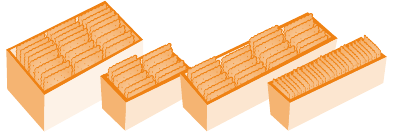
\includegraphics{./Images/galletas.png}
 % galletas.png: 393x133 pixel, 96dpi, 10.40x3.52 cm, bb=0 0 295 100
\end{center}
\item  ¿Cuáles serían las posibles distribuciones si las cajas contienen
40 galletas? Represéntalas
\end{enumerate}
\section*{¿Conoces los números primos?}
\subsection*{Lo que sé}
Resuelve individualmente

\begin{minipage}[]{.55\textwidth}
En el criadero de reptiles también tienen lagartos de diferentes especies. Uno de ellas es el lagarto arlequín que pone entre 30 y 40 huevos de forma alargada.

Una mañana Juan recogió huevos de dos hembras de esta especie. Una de ellas tenía 36 huevos y la otra 37. Cada grupo de huevos debía acomodarse en una cubeta como la de la figura. 
\end{minipage} \hfill
\begin{minipage}{.35\textwidth}
 \begin{center}
 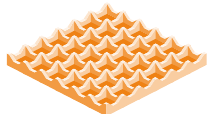
\includegraphics{./Images/cubeta.png}
 % cubeta.png: 211x114 pixel, 96dpi, 5.58x3.02 cm, bb=0 0 158 85
\end{center}
\end{minipage}
\begin{itemize}
 \item ¿Qué grupo de huevos puede acomodar Juan en las cubetas,
sin que le sobren? Explica
\end{itemize}
\subsection*{Aprende algo nuevo}
Con los 36 huevos se puede hacer un arreglo de 6 filas en el que cada fila tenga exactamente 6 huevos.
\begin{itemize}
\begin{minipage}{.55\textwidth}
\item  ¿36 es divisible por 6? ¿Por qué?
 \item  Con el grupo de 37 huevos, ¿se puede formar un arreglo
de seis filas, cada una con igual número de huevos?
 \item ¿Se utilizarían todos los huevos? ¿Cuántos sobran?
 \item Representa en tu cuaderno la situación.
 \item  ¿Por qué Juan no pudo acomodar los 37 huevos en una sola bandeja?
\end{minipage}\hfill
\begin{minipage}{.35\textwidth}
 \begin{center}
 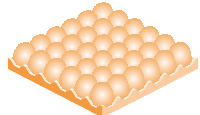
\includegraphics{./Images/huevos_01.png}
 % huevos_01.png: 200x115 pixel, 96dpi, 5.29x3.04 cm, bb=0 0 150 86
\end{center}
\end{minipage}
\item ¿37 es divisible por 6? ¿Por qué?
\item ¿Cuándo un número es divisible por otro?
\item ¿Recuerdas cuáles son los factores de 36? Escríbelos.
\item Ahora halla los factores de 37.
\item ¿Cuáles son?
\item ¿El número 36 es primo o es compuesto? ¿Por qué?
\item ¿El número 37 es primo o es compuesto? ¿Por qué?
\end{itemize}
En tu cuaderno, realiza divisiones para comprobar si:
\begin{itemize}
\begin{multicols}{2}
 \item 36 es divisible entre 2
 \item 36 es divisible entre 3
 \item 36 es divisible entre 5
 \item 36 es divisible entre 10.
 \item ¿Cuáles divisiones fueron exactas?
 \end{multicols}
 \item ¿En cuáles divisiones se obtuvo un residuo diferente de cero?
\end{itemize}
Sigue el mismo procedimiento para comprobar que los números 32, 64, 96, 108 y 200 son divisibles entre 2.

Los números 32, 64, 96, 108 y 200, ¿son pares o impares?\\
¿Por qué sabes que son pares o que son impares?

Responde en tu cuaderno, ¿cuándo un número es divisible entre 2?\\

Compara lo que escribiste con lo que aparece a continuación:

\emph{Un número es divisible por 2 si el dígito de las unidades es 0, 2, 4, 6, 8.}

Este enunciado se conoce como criterio de divisibilidad entre 2.
\begin{itemize}
\begin{multicols}{2}
 \item  ¿596 es divisible por 2? ¿Por qué?
 \item ¿129 es divisible por 2? ¿Por qué? 
 \end{multicols}
 \item Ahora analiza cuándo un número es divisible por 3.
 \begin{multicols}{2}
 \item ¿18 es múltiplo de 3?
 \item ¿18 es divisible entre 3?
 \item ¿24 es múltiplo de 3?
 \item ¿24 es divisible entre 3?
 \item ¿Cuáles cifras forman el número 18?
 \item ¿Cuál es la suma de esas cifras?
 \item ¿Es 9 divisible por 3?
 \item ¿Cuáles cifras forman el número 24?
 \item ¿Cuál es la suma de esas cifras?
 \item ¿Es 6 divisible por 3?
 \end{multicols}
\end{itemize}

\end{document}
